\section{Sets and Numbers}
In this section, we learn one of the two most fundamental concepts of mathematics, the \emph{set}. Much of what we cover in this unit will be material you already know from arithmetic and beginning algebra classes, but using the language of sets, and stating some of the rules more formally. Our main focus here is on the \emph{language}, rather than on the facts that it conveys.

This section is substantially longer than most of the sections in the course, because it contains a substantial amount of review material. Later sections will contain less material, but will require more practice to learn new skills.

\subsection{Introducing Sets} 
Sets are one of the fundamental concepts of mathematics, but it turns out to be remarkably difficult to define them precisely. Here's an informal definition:
\begin{definition}[Set (informal)]
A \term{set} is a collection of (usually mathematical) objects. The objects in a set are called its \term{elements}.
\end{definition}
This definition is not helpful. Let's see some examples.
\begin{example}
We can have a set containing the numbers 1, 2, and 3. We would write this as $\{1,2,3\}$. We could also give it a name, for example, $A=\{1,2,3\}$.
\end{example}
Key things to notice about this:
\begin{itemize}
\item There are \makeblanksmall numbers in this set: \makeblanksmall, \makeblanksmall, and \makeblanksmall.
\item However, this is \makeblanksmall set, named \makeblanksmall.
\item Think of the set as a ``container'' full of numbers.
\item The number $2$ is an \makeblank of the set \makeblanksmall (it's one of the numbers on the list). To indicate this, we can write $2\in A$.
\item The number $5$ is \emph{not} an \makeblank of the set \makeblanksmall (because it's not one of the numbers on the list). To indicate this, we can write $5\notin A$.
\end{itemize}
When we talk about sets, \makeblank doesn't matter. We could list this set as any of:
\begin{align*}
A&=\{1,2,3\}&
A&=\{1,3,2\}&
A&=\{2,1,3\}\\
A&=\{2,3,1\}&
A&=\{3,1,2\}&
A&=\{3,2,1\}
\end{align*}
It's also the case that \makeblank doesn't matter. All of these are also the same set:
\begin{align*}
A&=\{1,2,3\}&
A&=\{1,1,2,3\}&
A&=\{1,2,2,3,3,3,1\}
\end{align*}
All that matters is whether a number \emph{is} or \emph{is not} in the set.
\subsection{Roster Notation} 
Previously, we listed a set
\[
A=\{1,2,3\}
\]
This set is given in \emph{roster notation}.
\begin{definition}[Roster Notation]
A set is listed in \term{roster notation} by listing all of its elements, enclosed in \term{set brackets}.
\end{definition}
\begin{Note}Set brackets are curly. Here's how to write them.
\begin{cpic}{}{2}
\end{cpic}
\end{Note}
For larger sets, it's not always practical (or possible!) to list all of the elements. In this case, we use \makeblank to shortcut how they're written.
\begin{Note}
The \makeblank in which we write the elements of the set still doesn't matter, it is important to see the pattern.
\end{Note}
\begin{Example}
The set $\{1,2,3,\dots,10\}$ consists of \makeblank[1in] numbers from \makeblanksmall to \makeblanksmall. If we wrote out the entire set, it would be:
\[
\makeblank[3in]
\]
\end{Example}
\begin{Example}
The set $\{2,4,6,\dots,100\}$ consists of \makeblank[1in] numbers from \makeblanksmall to \makeblanksmall. (We won't write out the entire set here.)
\end{Example}
We can also use three dots at the end to mean the set ``goes on forever.''
\begin{Example}
The set $\{3,6,9,12,\dots\}$ contains \emph{all} the numbers that we get counting by \makeblank[1in].
\end{Example}
It should be \emph{easy} to make sense of the pattern.
%\begin{Example}
%If we wrote $\{3,6,9,\dots,100\}$, the pattern doesn't make sense:
%\begin{itemize}
%\item We are counting by \makeblank[1in]
%\item But if we continue that pattern, we would count \makeblanksmall followed by \makeblanksmall and miss $100$ entirely!
%\end{itemize}
%If we rewrite this set as
%\[
%\makeblank[3in]
%\]
%we have a set that makes sense.
%\end{Example}
\begin{Example}
If we write $\{1,3,7,\dots\}$ it isn't obvious what the pattern is.
\begin{itemize}
\item The pattern might be: add \makeblanksmall, add \makeblanksmall, so next we would add \makeblanksmall to get \makeblanksmall as our next number.
\item The pattern might also be: \makeblank[1in] the number add add \makeblanksmall, so the next number would be \makeblank.
\item Maybe you can spot other possible patterns, too!
\end{itemize}
In a case like this, we might be better off to use \emph{set-builder notation}, which we'll meet later.
\end{Example}
\subsection{Natural Numbers and Whole Numbers} 
There are several standard sets of numbers we discuss in mathematics. We build them up formally in the same way we built them up informally as we first learned about numbers.
\begin{definition}[Natural Numbers]
The \term{natural numbers} (sometimes called the \term{counting numbers}) are the set
\[
\mathbb{N}=\{1,2,3,\dots\}
\]
\end{definition}
\begin{itemize}
\item The natural numbers are all \makeblank
\item They do not have any \makeblank parts
\end{itemize}
The natural numbers are the numbers that give an intuitive answer to ``how many?'' questions. We can add in one more (less intuitive) answer to such a question, and our math gets much more powerful.
\begin{definition}[Whole Numbers]
The \term{whole numbers} are the set
\[
\mathbb{W}=\{0,1,2,3,\dots\}
\]
The difference from the natural numbers is the number \makeblanksmall
\end{definition}
\begin{Note}
The number $0$ is \emph{not} considered a \makeblank number. (It isn't a \makeblank number, either---it's in a cateogry of its own.)
\end{Note}
\begin{Example}
Which of these numbers are natural numbers? Whole numbers?
\begin{itemize}
\item $-2$ \checkbox{Natural Number} \checkbox{Whole Number}
\makeblanknew
\item $0$ \checkbox{Natural Number} \checkbox{Whole Number}
\makeblanknew
\item $3$ \checkbox{Natural Number} \checkbox{Whole Number}
\makeblanknew
\item $\frac{10}{5}$ \checkbox{Natural Number} \checkbox{Whole Number}
\makeblanknew
\item $\frac{11}{5}$ \checkbox{Natural Number} \checkbox{Whole Number}
\makeblanknew
\end{itemize}
\end{Example}
\subsection{Integers} 
\begin{definition}[Integers]
The \term{integers} are the set
\[
\mathbb{Z}=\{\dots,-3,-2,-1,0,1,2,3,\dots\}
\]
Note that this set continues forever in \makeblank[1in] directions.
\end{definition}
\begin{note}
We use the letter $\mathbb{Z}$ for the integers, not the letter $\mathbb{I}$. That's because we'll use $\mathbb{I}$ later.
\end{note}
\begin{itemize}
\item The integers include the \makeblank[1.5in] natural numbers, \makeblanksmall, and the \makeblank[1.5in] versions of the natural numbers.
\item They still have no \makeblank[1.5in] part.
\end{itemize}
\begin{example}
Which of these numbers are natural numbers? Whole numbers? Integers?
\begin{itemize}
\item $-5$ \checkbox{Natural Number} \checkbox{Whole Number} \checkbox{Integer}
\makeblanknew
\item $-1.3$ \checkbox{Natural Number} \checkbox{Whole Number} \checkbox{Integer}
\makeblanknew
\item $0$ \checkbox{Natural Number} \checkbox{Whole Number} \checkbox{Integer}
\makeblanknew
\item $3$ \checkbox{Natural Number} \checkbox{Whole Number} \checkbox{Integer}
\makeblanknew
\item $3\frac{1}{3}$ \checkbox{Natural Number} \checkbox{Whole Number} \checkbox{Integer}
\makeblanknew
\end{itemize}
\end{example}
\subsection{Set Builder Notation} 
If we have a set that's hard to describe in roster notation, we use an alternate notation.
\begin{definition}[Set-Builder Notation]
A set written in \term{set-builder notation} has the following form:
\[
\left\{\mbox{form of a set element} \mid \mbox{rules variables must follow}\right\}
\]
\end{definition}
\begin{Example}
The set
\[
\left\{
\frac{n}{2}
\mid
n\mbox{ is a natural number less than 10}
\right\}
\]
is the set
\[
\makeblank[3in]
\]
\end{Example}
\begin{Note}
We read this as ``the set of all (elements) such that (rule).'' For example, $\left\{x\mid x<10\right\}$ would be read as:\makeblanknew
\end{Note}

\subsection{Rational Numbers}
We'll use set-builder notation to define the next set of numbers.
\begin{definition}[Rational Numbers]
The \term{rational numbers} are the set
\[
\mathbb{Z}=\left\{\frac{n}{d}\mid n,d\mbox {are integers and }d\neq 0\right\}
\]
Any number which \emph{can} be written in this form is a rational number.
\end{definition}
We need a few notes on rational numbers, and a couple more definitions.
\begin{itemize}
\item Every integer is a rational number, because for an integer $n$ we can write\linebreak$n=\makeblanksmall$.
\item We can think of the fraction $\frac{n}{d}$ as the result of $n\div d$.
\item Note that the numerator $n$ can be 0, but the denominator $d$ cannot, because we can't \makeblank[1in] by 0.
\item A fraction can also be expressed as a \makeblank.
\end{itemize}
\begin{Example}
Which of these numbers are whole numbers? Integers? Rational numbers?
\begin{itemize}
\item $-\frac{2}{3}$ \checkbox{Whole Number} \checkbox{Integer} \checkbox{Rational Number}
\makeblanknew
\item $-6$ \checkbox{Whole Number} \checkbox{Integer} \checkbox{Rational Number}
\makeblanknew
\item $0$ \checkbox{Whole Number} \checkbox{Integer} \checkbox{Rational Number}
\makeblanknew
\item $\frac{7}{2}$ \checkbox{Whole Number} \checkbox{Integer} \checkbox{Rational Number}
\makeblanknew
\item $\pi$ \checkbox{Whole Number} \checkbox{Integer} \checkbox{Rational Number}
\makeblanknew
\end{itemize}
\end{Example}
We can organize the number sets so far:
\begin{center}
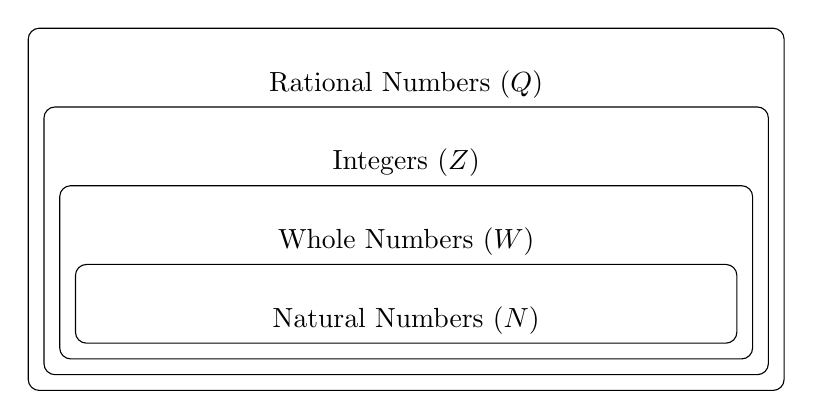
\begin{tikzpicture}
\foreach \x in {1,2,3,4}
	\draw[rounded corners] (-4-\x/5,0.2-\x/5) rectangle (4+\x/5,\x);
\draw (0,0.2) node[anchor=base] {Natural Numbers ($\mathbb{N}$)};
\draw (0,1.2) node[anchor=base] {Whole Numbers ($\mathbb{W}$)};
\draw (0,2.2) node[anchor=base] {Integers ($\mathbb{Z}$)};
\draw (0,3.2) node[anchor=base] {Rational Numbers ($\mathbb{Q}$)};
\end{tikzpicture}
\end{center}
\subsection{Simplifying Fractions}
There are \makeblank to write any rational number as a fraction.
\begin{definition}[Equivalent Fractions]
Two fractions $\frac{a}{b}$ and $\frac{c}{d}$ are \term{equivalent} if
$$
ad=bc
$$
The products $ad$ and $bc$ are called the \term{cross-products}. If $\frac{a}{b}$ and $\frac{c}{d}$ are equivalent, we write
$$
\tfrac{a}{b}=\tfrac{c}{d}
$$
and think of the fractions as representing the same rational number.
\end{definition}
This definition helps us check whether fractions are equivalent, but doesn't help us get equivalent fractions.
\begin{itemize}
\item For any \makeblank[1in] $c\neq\makeblanksmall$, $\frac{a}{b}=\frac{a\cdot c}{b\cdot c}$
\item For any \makeblank[1in] $c$ such that $a\div c$ and $b\div c$ are both \makeblank[1in] (that is, $c$ is a \makeblank of $a$ and $b$), $\frac{a}{b}=\frac{a\div c}{b\div c}$.
\end{itemize}
\begin{definition}[Lowest Terms]
A fraction $\frac{n}{d}$ is said to be in \term{lowest terms} if
\begin{itemize}
\item $n$ and $d$ have no common factors except \makeblanksmall and \makeblanksmall
\item \makeblanksmall is positive
\end{itemize}
Every fraction is equivalent to \makeblank fraction in lowest terms. The process of putting a fraction in lowest terms is called \term{simplifying} or \term{reducing} the fraction.
\end{definition}
\begin{example}
Simplify the fraction $\frac{-18}{-42}$
\begin{cpic}{}{5}
\end{cpic}
\end{example}
If we use a \makeblank for fraction arithmetic, it automatically gives the result in lowest terms.
\subsection{Review of Fraction Arithmetic}
To add fractions:
\begin{itemize}
\item Write equivalents that have the same \makeblank[1in].
\item Add the \makeblank[1in]
\item Simplify, if necessary.
\end{itemize}
\begin{example}
Add $\frac{3}{4}+\frac{1}{6}$
\begin{cpic}{}{4}
\end{cpic}
\end{example}
To multiply fractions:
\begin{itemize}
\item Multiply the \makeblank[1in]
\item Multiply the \makeblank[1in]
\item Simplify, if necessary.
\end{itemize}
\begin{example}
Multiply $\frac{3}{8}\times\frac{10}{9}$
\begin{cpic}{}{2}
\end{cpic}
\end{example}
We can also use a \makeblank[1in] for fraction arithmetic.
\begin{itemize}
\item On the TI-84:
\begin{itemize}
\item To enter a fraction, press \makeblank[.75in] \makeblank[.75in] \makeblank[.75in] 
\item To enter a mixed number, press \makeblank[.75in] \makeblank[.75in] \makeblank[.75in] 
\item To output a fraction, press \makeblank[.75in] \makeblank[.75in]
\item To convert a fraction to a mixed number, press \makeblank[.75in] \makeblank[.75in]
\end{itemize}
\item On the TI-30XS:
\begin{itemize}
\item To enter a fraction, press \makeblank[.75in]
\item To enter a mixed number, press \makeblank[.75in] \makeblank[.75in] 
\item To convert output to a fraction, press \makeblank[.75in] 
\item To convert a fraction to a mixed number, press \makeblank[.75in] \makeblank[.75in] 
\end{itemize}
\end{itemize}
\subsection{Decimals and Fractions}
A fraction can also be expressed as a \makeblank.
\begin{theorem}
Every fraction can be expressed as either a terminating or repeating decimal. Every terminating and repeating decimal can be expressed as a fraction.
\end{theorem}
\begin{proof}
To write a fraction $\frac{n}{d}$ as a decimal, perform the division $n\div d$. In the process of long division, we will always reach a point where the remainder is either zero, or repeats itself.

To write a terminating decimal as a fraction, write the decimal as $\frac{w}{10^n}$, where $w$ is the number obtained by deleting the decimal point and $n$ is the number of digits after the decimal point.

To write a repeating decimal as a fraction, use the algebra process demonstrated below.
\end{proof}
\begin{example}
Write each fraction as a decimal.
\begin{itemize}
\item $\frac{3}{5}=\makeblanksmall$
\item $\frac{5}{11}=\makeblanksmall$
\item $\frac{7}{12}=\makeblanksmall$
\end{itemize}
\end{example}
\begin{example}
Write each decimal as a fraction.
\begin{itemize}
\item $2.25=\makeblank[1in]$
\item $0.3\overline{18}=\makeblank[1in]$
\end{itemize}
\begin{lpic}{}{10}
\regtextleft{0}{-1}{Let $x=$};
\regtextleft{1}{-2}{digit before repeating, so multiply by};
\regtextleft{1}{-4}{digits repeat, so multiply by};
\regtextleft{0}{-7}{Subtract to eliminate the repeating part};
\end{lpic}
\end{example}
\subsection{Irrational Numbers and Real Numbers}
Of the numbers on the number line, not all are rational.
\begin{definition}[Real numbers]
A number that cannot be written as a fraction is called \term{irrational}. The rational numbers combined with the irrational numbers make up the \term{real numbers}, represented by the symbol $\mathbb{R}$. The real numbers make up all of what we think of as ``numbers.''
\end{definition}
What are these irrational numbers, anyway?
\begin{example}
The number $0.10110011100011110000\dots$ is irrational. This decimal does not \makeblank[1in] or \makeblank[1in].
\end{example}
\begin{example}
The number $\sqrt{2}$ is irrational. In fact, for any whole number $n$, $\sqrt{n}$ is either a whole number or irrational.
\end{example}
\begin{example}There are also some numbers that are defined to work in formulas that turn out to be irrational, such as the number $\pi$, which is defined to work in the formula $C=2\pi r$ for the \makeblank of a circle.
\end{example}
\begin{example}
Which of these numbers are Whole numbers? Integers? Rational numbers?
\begin{itemize}
\item $-2.3$ \checkbox{Rational Number} \checkbox{Irrational Number} \checkbox{Real Number}
\makeblanknew
\item $\sqrt{5}$ \checkbox{Rational Number} \checkbox{Irrational Number} \checkbox{Real Number}
\makeblanknew
\item $\sqrt{9}$ \checkbox{Rational Number} \checkbox{Irrational Number} \checkbox{Real Number}
\makeblanknew
\item $\pi$ \checkbox{Rational Number} \checkbox{Irrational Number} \checkbox{Real Number}
\makeblanknew
\end{itemize}
\end{example}
We can organize all of our number sets:
\begin{center}
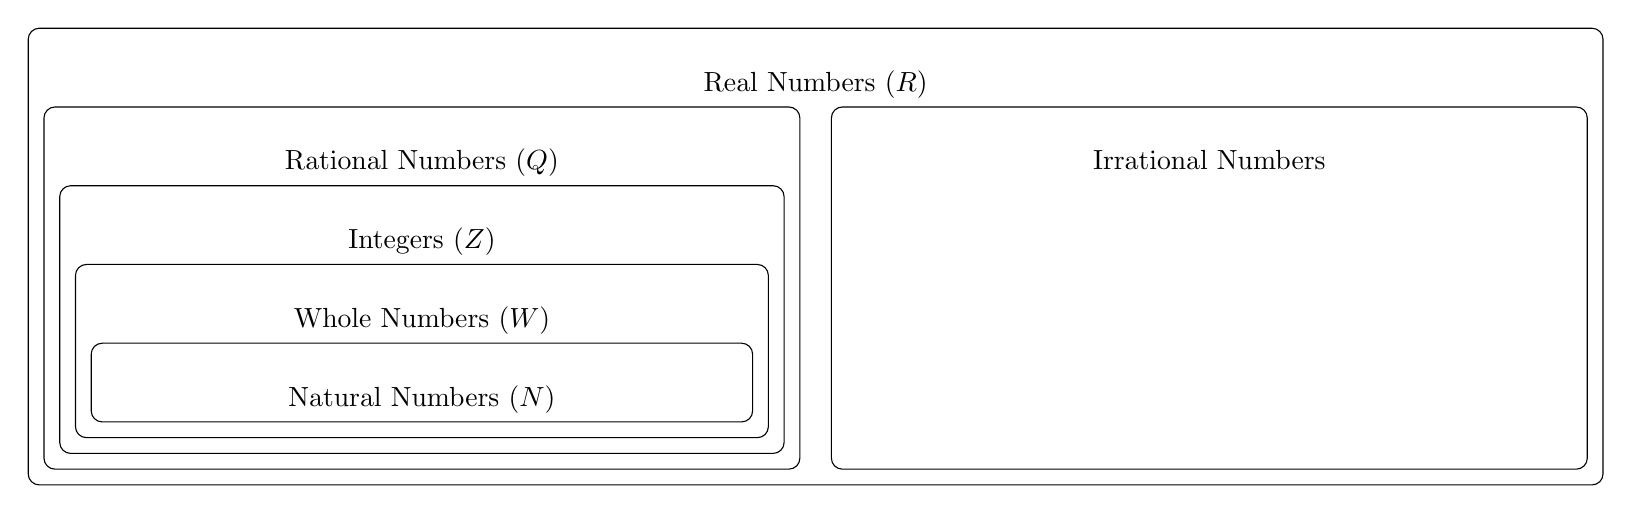
\begin{tikzpicture}
\foreach \x in {1,2,3,4}
	\draw[rounded corners] (-4-\x/5,0.2-\x/5) rectangle (4+\x/5,\x);
\draw (0,0.2) node[anchor=base] {Natural Numbers ($\mathbb{N}$)};
\draw (0,1.2) node[anchor=base] {Whole Numbers ($\mathbb{W}$)};
\draw (0,2.2) node[anchor=base] {Integers ($\mathbb{Z}$)};
\draw (0,3.2) node[anchor=base] {Rational Numbers ($\mathbb{Q}$)};
\draw[rounded corners] (5.2,-0.6) rectangle (14.8,4);
\draw (10,3.2) node[anchor=base] {Irrational Numbers};
\draw[rounded corners] (-5,-0.8) rectangle (15,5);
\draw (5,4.2) node[anchor=base] {Real Numbers ($\mathbb{R}$)};
\end{tikzpicture}
\end{center}
\subsection{Properties of Addition and Multiplication} 
Addition and multiplication have some useful properties on our number sets.
\begin{displaybox}[Properties of Addition and Multiplication]
\begin{itemize}
For any three real numbers $a$, $b$, and $c$, we have the following properties.
\item Addition and multiplication are \makeblank[1.5in]:
\[
a+b=b+a
\qquad
ab=ba
\]
\item Addition and multiplication are \makeblank[1.5in]:
\[
(a+b)+c=a+(b+c)
\qquad
(ab)c=a(bc)
\]
Because of this, we can write sums or products of three (or more) numbers without parentheses.
\item The \makeblank[1.5in] property combines addition and multiplication:
\[
a(b+c)=ab+ac
\qquad
(b+c)a=ba+ca
\]
\end{itemize}
\end{displaybox}
\begin{displaybox}[Closure]
The natural numbers, the whole numbers, the integers, the rational numbers, and the real numbers are \term{closed} under multiplication and addition. That means:
\begin{itemize}
\item The sum or product of two natural numbers is a \makeblank[1in] number
\item The sum or product of two whole numbers is a \makeblank[1in] number
\item The sum or product of two integers is an \makeblank[1in]
\item The sum or product of two rational numbers is a \makeblank[1in] number
\item The sum or product of two real numbers is a \makeblank[1in] number
\end{itemize}
The sum or product of two irrational numbers could be rational or irrational, depending on the numbers. However:
\begin{itemize}
\item The sum of a rational number and an irrational number is an \makeblank[1in] number
\item The product of a \emph{nonzero} rational number and an irrational number is an \makeblank[1in] number.
\end{itemize}
\end{displaybox}
\subsection{Identity and Inverse} 
Here are some properties that only hold if we have ``big enough'' number sets.
\begin{displaybox}[Identity]
There is a number \makeblanksmall the \term{additive identity} such that, for any real number $a$,
\[
\makeblanksmall+a=a+\makeblanksmall=a
\]
There is also a number \makeblanksmall the \term{multiplicative identity} such that, for any real number $a$,
\[
\makeblanksmall\cdot a=a\cdot\makeblanksmall=a
\]
\end{displaybox}
So far, we've only talked about addition and multiplication, not subtraction and division. Why?
\begin{displaybox}[Inverse]
For any real number $a$, there is a number \makeblanksmall called its \term{additive inverse} such that
\[
a+\makeblanksmall = \makeblanksmall+a = 0
\]
For any real number $a$ \emph{except for zero}, there is a number \makeblanksmall called its \term{multiplicative inverse} such that
\[
a\cdot\makeblanksmall = \makeblanksmall\cdot a=1
\]
\end{displaybox}
\begin{Note}
We wrote the multiplicative inverse of a number $a$ as $\frac{1}{a}$, but in general, to find the multiplicative inverse, we take the \makeblank[1.5in] of the number.
\begin{itemize}
\item The multiplicative inverse of $4$ is \makeblanksmall
\item The multiplicative inverse of $\frac{2}{3}$ is \makeblanksmall
\end{itemize}
\end{Note}
\begin{definition}[Subtraction and Division]
We define a new operation, \term{subtraction}, based on addition, by
\[
a-b=\makeblanksmall + \makeblanksmall
\]
We define a new operation, \term{division}, based on multiplication, by
\[
a\div b=\makeblanksmall\cdot\makeblanksmall
\]
\end{definition}

%\input{Functions/Sets/Some Algebraic Structures}
\subsection{Properties of Exponents} 
As well as addition and multiplication, we have a third ``operation'' that is (at the moment) designed only for some numbers.
\begin{definition}[Exponent]
For any real number $x$ and natural number $n$, the expression $x^n$ is defined as repeated multiplication.
\[
x^n=\underbrace{x\cdot x\cdots x}_{\text{$n$ copies}}
\]
The number $x$ is called the \term{base}, and the number $n$ is called the \term{exponent}.
\end{definition}
\begin{itemize}
\item We can read $x^2$ as ``$x$ \makeblank[1in]'' or ``$x$ to the second.''
\item We can read $x^3$ as ``$x$ \makeblank[1in]'' or ``$x$ to the third.''
\item For any other number $n$, we read $x^n$ as ``$x$ to the power $n$'' or ``$x$ to the $n$th power.''
\end{itemize}
We have certain properties of exponents, which are easy to see for natural number exponents.
\begin{displaybox}[Powers of the Same Base]
For any real number $x$ and natural numbers $m$, $n$, and $p$, with $m\geq n$, we have:
\[
x^m\cdot x^n = x^{m+n}
\qquad
\frac{x^m}{x^n}=x^{m-n}
\qquad
\frac{x^n}{x^m}=\frac{1}{x^{n-m}}
\qquad
\left(x^n\right)^p=x^{np}
\]
\end{displaybox}
\begin{Example}
Rewrite each expression with a single exponent.
\begin{lpic}{}{2}
\twocolleft{-1}{2}{$x^3\cdot x^5=$}{$\frac{t^5}{t^2}=$}
\twocollblleft{-2}{$\frac{3^{11}}{3^{29}}=$}{$\left(k^4\right)^5=$}
\end{lpic}
%\begin{itemize}
%\item $x^3\cdot x^5=\makeblank$
%\item $\dfrac{t^5}{t^2}=\makeblank$
%\item $\dfrac{3^{11}}{3^{29}}=\makeblank$
%\item $\left(k^4\right)^5=\makeblank$
%\end{itemize}
\end{Example}
\begin{displaybox}[Powers of Products and Quotients]
For any real numbers $x$, $y$, and $z$, with $z\neq 0$, and natural number $n$, we have:
\[
\left(xy\right)^n=x^ny^n
\qquad
\left(\frac{x}{z}\right)^n=\frac{x^n}{z^n}
\]
\end{displaybox}
\begin{Example}
Rewrite each expression with a single exponent.
\begin{lpic}{}{1}
\twocolleft{-1}{1}{$\left(2x\right)^3=$}{$\left(\dfrac{x}{6}\right)^2=$}
\end{lpic}
\end{Example}
\subsection{Properties of Equality} 
\begin{displaybox}[Symmetric Property of Equality]
For any real numbers $a$ and $b$:
\[
a=b
\quad\mbox{if and only if}\quad
b=a
\]
\end{displaybox}
\begin{displaybox}[Transitive Property of Equality]
For any real numbers $a$, $b$, and $c$:
\[
\mbox{If }a=b\mbox{ and }b=c\mbox{ then }a=c
\]
\end{displaybox}
\begin{displaybox}[Additive Property of Equality]
For any real numbers $a$, $b$, and $c$:
\[
a=b
\quad\mbox{if and only if}\quad
a+c = b+c
\]
%This property means that we can get an ``equivalent equation'' by adding the same number to both sides. 
We will sometimes think of this as ``subtracting,'' but remember that subtracting is just adding the \makeblank[1.5in].
\end{displaybox}
\begin{displaybox}[Multiplicative Property of Equality]
For any real numbers $a$, $b$, and $c$, with $c\neq 0$:
\[
a=b
\quad\mbox{if and only if}\quad
ac=bc
\]
%This property means that we can get an ``equivalent equation'' by multiplying both sides by the same number, as long as it isn't zero. 
We will sometimes think of this as ``dividing,'' but remember that dividing is just multiplying by the \makeblank[1.5in].
\end{displaybox}
\begin{example}
Assume $2x+2=4x-6$. Manipulate the equation as follows:
\begin{lpic}{}{4}
\regtextleft{0}{-1}{Add $3$ to both sides};
\regtextleft{0}{-2}{Multiply both sides by $2$};
\regtextleft{0}{-3}{Subtract $3x$ from both sides};
\regtextleft{0}{-4}{Switch the order of the sides};
\end{lpic}
To check that these equations are all equivalent, we'll see that they're all true when $x=4$.
\begin{lpic}{}{3}
\end{lpic}
\end{example}
\subsection{Evaluating Expressions} 
To \emph{evaluate} an expression means to determine what number it represents. When the expression contains no variables, this is straight forward. With more than one operation, we follow the following order.
\begin{enumerate}
\item Grouping symbols---including \makeblank[1.5in] and \makeblank[1.5in]---come first. These are used to indicate that some operation comes out of order.
\item Exponents are evaluated before multiplication (or division). 
\item Multiplication (and \makeblank[1.5in]) come next. Note: \makeblank[1in] signs are at this level.
\item Addition (and \makeblank[1.5in]) come last.
\end{enumerate}
For complicated expressions, this is most easily done term-by-term.
\begin{Example}
Evaluate $\frac{(7-5)^3}{4}-9\div 3\cdot 7+8$
\begin{cpic}{}{5}
\end{cpic}
\end{Example}
Negative signs can create some confusion.
\begin{itemize}
\item $-5^2$ means first \makeblank[1in], then \makeblank[1in], so $-5^2=\makeblanksmall$
\item $(-5)^2$ means first \makeblank[1in], then \makeblank[1in], so $(-5)^2=\makeblanksmall$
\end{itemize}
When an expression contains variables, we must know what \makeblank[1in] the variables represent in order to evaluate.
\begin{Example}
Evaluate $3x^2-5xy+4y^2$ when $x=-2$ and $y=3$.
\begin{lpic}{}{4}
\regtextleft{0}{-1}{First we plug in:};
\end{lpic}
\end{Example}
\subsection{Simplifying Expressions} 
\begin{definition}[Simplify]
To \term{simplify} an expression means to manipulate it to get an \term{equivalent expression} in some standard form. Expressions are \term{equivalent} if they represent the same number, \emph{no matter what} the values of the variables.
\end{definition}
To learn to simplify a new kind of expression, you must learn:
\begin{itemize}
\item How to manipulate an expression of that kind.
\item What the standard form is.
\end{itemize}
We already know how to manipulate expressions in which variables are only added, subtracted, and multiplied by real numbers, which we call \makeblank[1in] expressions.
\begin{Example}
Simplify $3(2x-5)+4x-11z+5+5(z-1)$ as much as possible. Justify each step with one of the properties of real numbers.
\begin{cpic}{}{4}
\end{cpic}
To check that these expressions are equivalent, we can pick any two real numbers for $x$ and $z$. Let's choose $x=\makeblanksmall$ and $z=\makeblanksmall$.
\begin{lpic}{}{8}
\regtextleft{0}{-1}{$3(2x-5)+4x-11z+5+5(z-1)=$};
\regtextleft{0}{-6}{$10x-6z-15=$};
\end{lpic}
\end{Example}
\subsection{Solving Equations} 
\begin{definition}[Solution of an Equation]
A \term{solution} of an equation is a value (or values) of the variable (or variables) that make the equation \makeblank[1in].
\end{definition}
\begin{Example}
Confirm that $x=2$ is a solution to the equation $3x^2-5x-2=0$.
\begin{cpic}{}{2}
\end{cpic}
\end{Example}
\begin{definition}[Solve an Equation]
To \term{solve} an equation means to \emph{find} all the solutions to an equation, and also to \emph{demonstrate} that we have found all the solutions to the equation. To show that we have all the solutions, we must ``\makeblank.''
\end{definition}
Sometimes, we can solve an equation by \emph{inspection}: we look at the equation, and know the solution.
\begin{Example} Solve $x+4=10$.
\begin{itemize}
\item We know that $\makeblanksmall+4=10$, so the only solution must be $x=\makeblanksmall$.
\end{itemize}
\end{Example}
Otherwise, we need a process. We will expand on this process throughout the course.
\begin{displaybox}[Solve Any Equation]
To solve any equation, we might make the following moves.
\begin{enumerate}
\item Rewrite either side of the equation in different forms.
\item Use properties of equality to isolate parts of an expression.
\item ???
\item ???
\end{enumerate}
\end{displaybox}
\begin{Example}
Using the first two moves, solve the equation
\[
3(5x-7)=9
\]
in two different ways.
\begin{lpic}{}{4}
\twocolleft{-1}{4}{Method 1:}{Method 2:}
\end{lpic}
\end{Example}
